% Teilaufgabe 2

\section{Plasmon-Moden}

Oberflächenplasmonen (OP) lassen sich in der Regel nicht dur Licht anregen, da die Phasengeschwindigkeit nicht übereinstimmt und es sich bei OP um evaleszente Wellen handelt. Folglich stimmt der Wellenvektor nicht überein und es kommt keine Anregung zustande. Dies kann durch Verwendung von Prismeneinkoplung umgangen werden, hier wird unter Verwendung von Totalreflexion und der daraus resultierenden evaleszenten Welle, in Verbindung mit unterschiedlichen Lichtgeschwindigkeiten in zwei Dielektrika eine Einkopplung erreicht.

\begin{figure}[h]
    \centering
    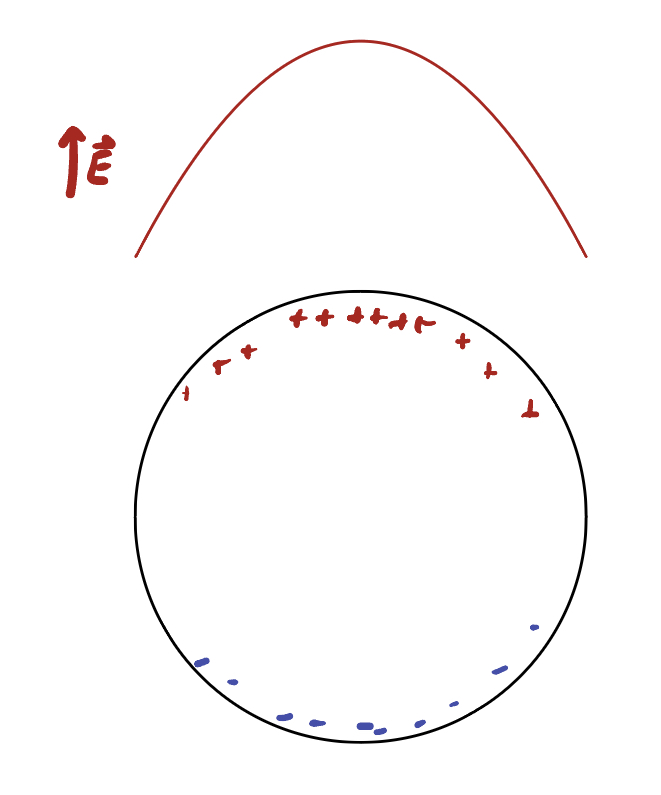
\includegraphics[width=0.25\textwidth]{Bilder/Grundmode.jpeg}
    \caption{Grundmode}
\end{figure}